% =========================================================
% PHAN 10 -- CAU 9: COMPARISON WITH LIBRARY IMPLEMENTATION
% =========================================================

\section{So sánh với thư viện
(Comparison with Library Implementation)}
\label{sec:library-comparison}

\subsection{Mục tiêu và thiết lập thực nghiệm}

Nhằm đánh giá kết quả của thuật toán hồi quy
tuyến tính tự triển khai, nhóm so sánh hai
phương pháp ước lượng tham số:

\begin{itemize}
    \item \textbf{NumPy Gradient Descent (Baseline):}
    Mô hình hồi quy tuyến tính được cài đặt
    bằng NumPy và tối ưu bằng thuật toán
    Gradient Descent (GD).

    \item \textbf{Scikit-learn Linear Regression
    (Improvement Model):}
    Mô hình sử dụng lớp
    \texttt{LinearRegression} của Scikit-learn
    để giải bài toán bình phương tối thiểu
    (Ordinary Least Squares).
\end{itemize}

Cả hai mô hình sử dụng cùng đặc trưng đầu vào
\texttt{gateway\_rtt\_avg\_ms} và biến mục tiêu
\texttt{rtt\_avg\_ms}, lần lượt biểu diễn
RTT trung bình đến Gateway và RTT trung bình
đến máy chủ đích.

NumPy GD được khởi tạo với các tham số
bằng $0$, sử dụng learning rate
$\gamma=0.01$ và thực hiện $1000$ vòng lặp.
Scikit-learn Linear Regression được
huấn luyện bằng phương thức \texttt{fit}
trên cùng tập dữ liệu.

Hai phương pháp được đánh giá thông qua
tham số hồi quy, chất lượng dự đoán
và hiệu quả tính toán.


\subsection{Kết quả tham số hồi quy}

Bảng~\ref{tab:library-comparison}
trình bày các tham số hồi quy và
chỉ số đánh giá trên tập kiểm tra.

\begin{table}[H]
    \centering
    \caption{So sánh hai phương pháp
    hồi quy tuyến tính đơn biến}
    \label{tab:library-comparison}
    \small

    \begin{tabular}{lrr}
        \toprule
        \textbf{Chỉ số}
        & \textbf{NumPy GD}
        & \textbf{Scikit-learn LR} \\
        \midrule

        Hệ số chặn $\theta_0$
        & 12.313184 & 12.314673 \\

        Hệ số góc $\theta_1$
        & 0.831447 & 0.830910 \\

        Test MSE ($\mathrm{ms}^2$)
        & 31.352016 & 31.351569 \\

        Test $R^2$
        & 0.020990 & 0.021004 \\

        \bottomrule
    \end{tabular}
\end{table}

Các phương trình dự đoán tương ứng là:

\[
    \hat{y}_{\mathrm{GD}}
    =12.313184+0.831447x,
\]

\[
    \hat{y}_{\mathrm{LR}}
    =12.314673+0.830910x.
\]

Hệ số hồi quy của hai mô hình gần tương đương.
Theo kết quả từ Scikit-learn Linear Regression,
khi Gateway RTT tăng $1$ ms, RTT dự đoán
đến máy chủ đích tăng khoảng $0.8309$ ms.
Đây là mối liên hệ thống kê,
không hàm ý quan hệ nhân quả.

Hình~\ref{fig:univariate-comparison}
minh họa dữ liệu kiểm tra và hai đường hồi quy
được ước lượng bởi NumPy GD và Scikit-learn
Linear Regression.

\begin{figure}[H]
    \centering
    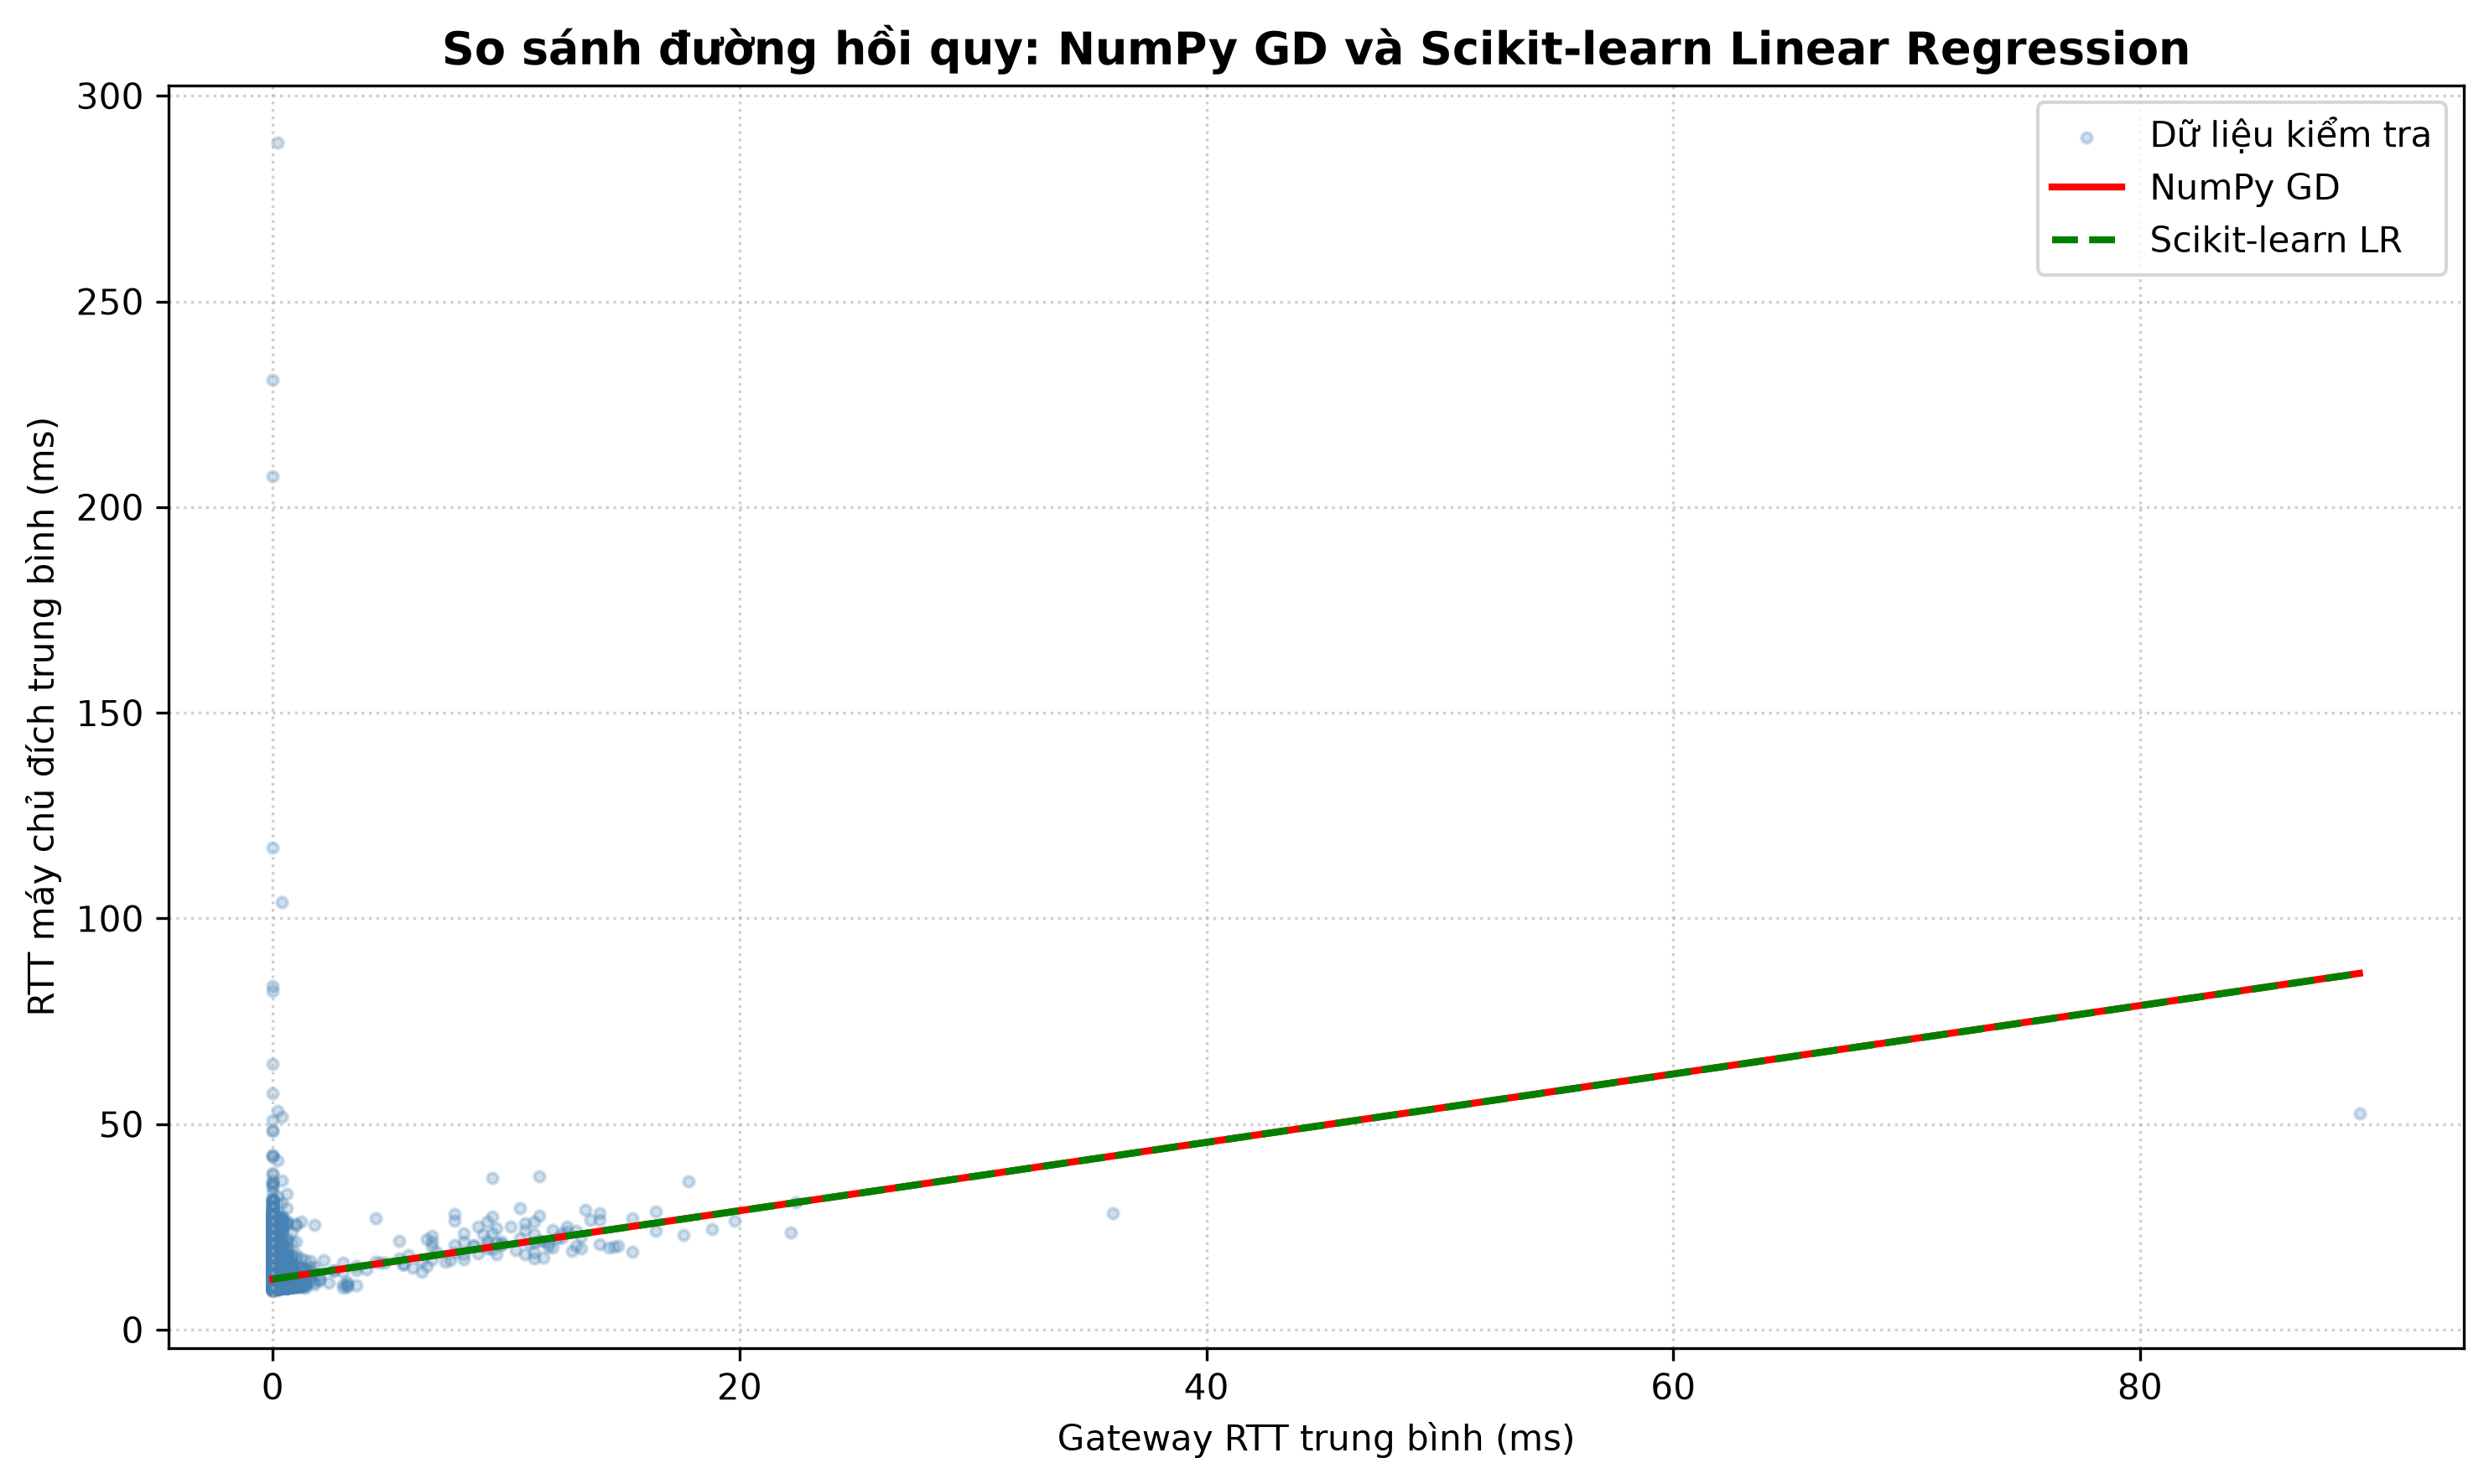
\includegraphics[
        width=0.95\textwidth
    ]{phan10.png}

    \caption{So sánh đường hồi quy của
    NumPy GD (Baseline) và
    Scikit-learn Linear Regression
    trên tập kiểm tra}
    \label{fig:univariate-comparison}
\end{figure}

Hai đường hồi quy gần như chồng khít,
cho thấy hai phương pháp tìm được
các bộ tham số có kết quả dự đoán
gần tương đương.

Tuy nhiên, các quan sát thực tế
phân tán đáng kể xung quanh đường hồi quy.
Đặc biệt, một số quan sát có RTT
đến máy chủ đích cao mặc dù
Gateway RTT ở mức thấp.

Điều này cho thấy chỉ sử dụng Gateway RTT
chưa đủ để biểu diễn toàn bộ mối quan hệ
giữa đặc trưng đầu vào và biến mục tiêu.

Đối với NumPy GD, hàm chi phí được sử dụng là:

\[
    J(\boldsymbol{\theta})
    =
    \frac{1}{2n}
    \sum_{i=1}^{n}
    (\hat{y}_i-y_i)^2.
\]

Trong khi đó, chỉ số MSE được định nghĩa:

\[
    \mathrm{MSE}
    =
    \frac{1}{n}
    \sum_{i=1}^{n}
    (\hat{y}_i-y_i)^2.
\]

Với cùng dữ liệu và bộ tham số:
\[
    \boxed{
        \mathrm{MSE}=2J(\boldsymbol{\theta})
    }.
\]

Hai hàm chỉ khác nhau bởi một hệ số dương
nên có cùng tập nghiệm cực tiểu.

Trong thí nghiệm, MSE của cả hai mô hình
đều được tính bằng
\texttt{mean\_squared\_error},
bảo đảm thống nhất định nghĩa chỉ số
khi đánh giá chất lượng dự đoán.


\subsection{Đánh giá hiệu năng dự đoán
và hiệu quả tính toán}

\paragraph{Inference Performance.}

Hiệu năng dự đoán được đánh giá trên
$10\,920$ quan sát kiểm tra,
sử dụng Mean Squared Error (MSE)
và hệ số xác định $R^2$:

\[
    \mathrm{MSE}
    =
    \frac{1}{m}
    \sum_{i=1}^{m}
    (y_i-\hat{y}_i)^2,
\]

\[
    R^2
    =
    1-
    \frac{
        \sum_{i=1}^{m}(y_i-\hat{y}_i)^2
    }{
        \sum_{i=1}^{m}(y_i-\bar{y})^2
    },
\]

trong đó $m$ là số mẫu kiểm tra
và $\bar{y}$ là giá trị trung bình
của biến mục tiêu trên tập kiểm tra.

Scikit-learn Linear Regression đạt
$\mathrm{MSE}=31.351569$,
thấp hơn NumPy GD khoảng
$0.000447\,\mathrm{ms}^2$.

Hệ số xác định của hai mô hình
đều xấp xỉ $0.021$.
Kết quả cho thấy chất lượng dự đoán
của hai phương pháp gần tương đương,
nhưng chỉ giải thích được khoảng
$2.1\%$ biến thiên của RTT
trên tập kiểm tra.

\paragraph{Computational Efficiency.}

Hiệu quả tính toán được đánh giá
thông qua thời gian huấn luyện,
sử dụng \texttt{time.perf\_counter()}.

Hai mô hình được huấn luyện lại
trên cùng tập dữ liệu $7$ lần.
Thời gian được tính từ khi bắt đầu
đến khi kết thúc quá trình huấn luyện,
không bao gồm bước dự đoán
và đánh giá chỉ số.

Thời gian trung vị được sử dụng
để tổng hợp kết quả các lần đo.

\begin{table}[H]
    \centering
    \caption{So sánh thời gian huấn luyện}
    \label{tab:library-training-time}
    \small

    \begin{tabular}{lrr}
        \toprule
        \textbf{Mô hình}
        & \textbf{Số lần đo}
        & \textbf{Trung vị (s)} \\
        \midrule

        NumPy GD (Baseline)
        & 7 & 0.090847 \\

        Scikit-learn Linear Regression
        & 7 & 0.00208639 \\

        \bottomrule
    \end{tabular}
\end{table}

Tỷ số thời gian huấn luyện là:

\[
    S=
    \frac{T_{\mathrm{GD}}}{T_{\mathrm{LR}}}
    =
    \frac{0.090847}{0.00208639}
    \approx43.54.
\]

Trong môi trường thực nghiệm,
Scikit-learn Linear Regression có
thời gian huấn luyện trung vị thấp hơn
NumPy GD khoảng $43.54$ lần.

Sự khác biệt này phù hợp với đặc điểm
triển khai của hai phương pháp.
NumPy GD thực hiện $1000$ bước
cập nhật gradient, trong khi
Scikit-learn Linear Regression sử dụng
bộ giải bình phương tối thiểu được
tối ưu hóa bằng các thư viện
đại số tuyến tính.

Tỷ số trên phản ánh kết quả đo
trong cấu hình thực nghiệm hiện tại,
không phải hệ số tăng tốc cố định
cho mọi dữ liệu hoặc môi trường tính toán.


\subsection{Nhận xét}

NumPy GD (Baseline) và Scikit-learn
Linear Regression (Improvement Model)
đạt chất lượng dự đoán gần tương đương,
với các hệ số hồi quy và MSE
chỉ chênh lệch rất nhỏ.

Sau $1000$ vòng lặp, thuật toán GD
tự triển khai đã tìm được bộ tham số
gần nghiệm bình phương tối thiểu.

Scikit-learn Linear Regression có lợi thế
rõ rệt về thời gian huấn luyện,
trong khi chất lượng dự đoán
gần như không thay đổi.

Tuy nhiên, hệ số xác định thấp
và độ phân tán của các quan sát
quanh đường hồi quy cho thấy giới hạn
của mô hình tuyến tính đơn biến.




Các kết quả trên xác nhận sự tương đương về dự đoán giữa
Gradient Descent và nghiệm bình phương tối thiểu trong bài toán
đơn biến. Để khảo sát tác động của số lượng đặc trưng và lựa chọn
thuật toán, Phần~\ref{sec:model-improvement} huấn luyện lại hai
mô hình đơn biến trên cùng tập dữ liệu với các mô hình đa biến.
Thiết kế này bảo đảm phép so sánh chín mô hình sử dụng cùng các
quan sát kiểm tra thay vì đối chiếu trực tiếp những chỉ số thu
được từ hai phép chia dữ liệu khác nhau.